\section{Vous êtes prêts ?}

Date: 13/11/2010

\begin{multicols}{2}

Bonjour,

C'est avec une certaine excitation que j'écris un nouveau message sur ce blog, mon sac est prêt, je repars pour un nouveau voyage le sac sur le dos, porté par les rencontres, la météo et les possibilités de transport locales.

La destination ? Une petite île à coté de l'Afrique.. Je vais à Madagascar pour trois semaines et demi.

Quant au programme, je suis encore incapable de vous le donner. Je vais attérir à Antananarivo vers le centre de l'île. Je pense ensuite descendre vers le Sud suivant les possibilités et remonter vers le nord pour la fin du voyage avant de redescendre vers la capitale. Comme d'habitude ce n'est qu'une prévision qui a toutes les chances d'être changée une fois là bas. Vous découvrirez donc la suite lorsque je la connaîtrai..

Ci-dessous une carte de l'île pour vous repérer dans les noms des villes que seront indiqués.

\hspace*{-0.65cm}
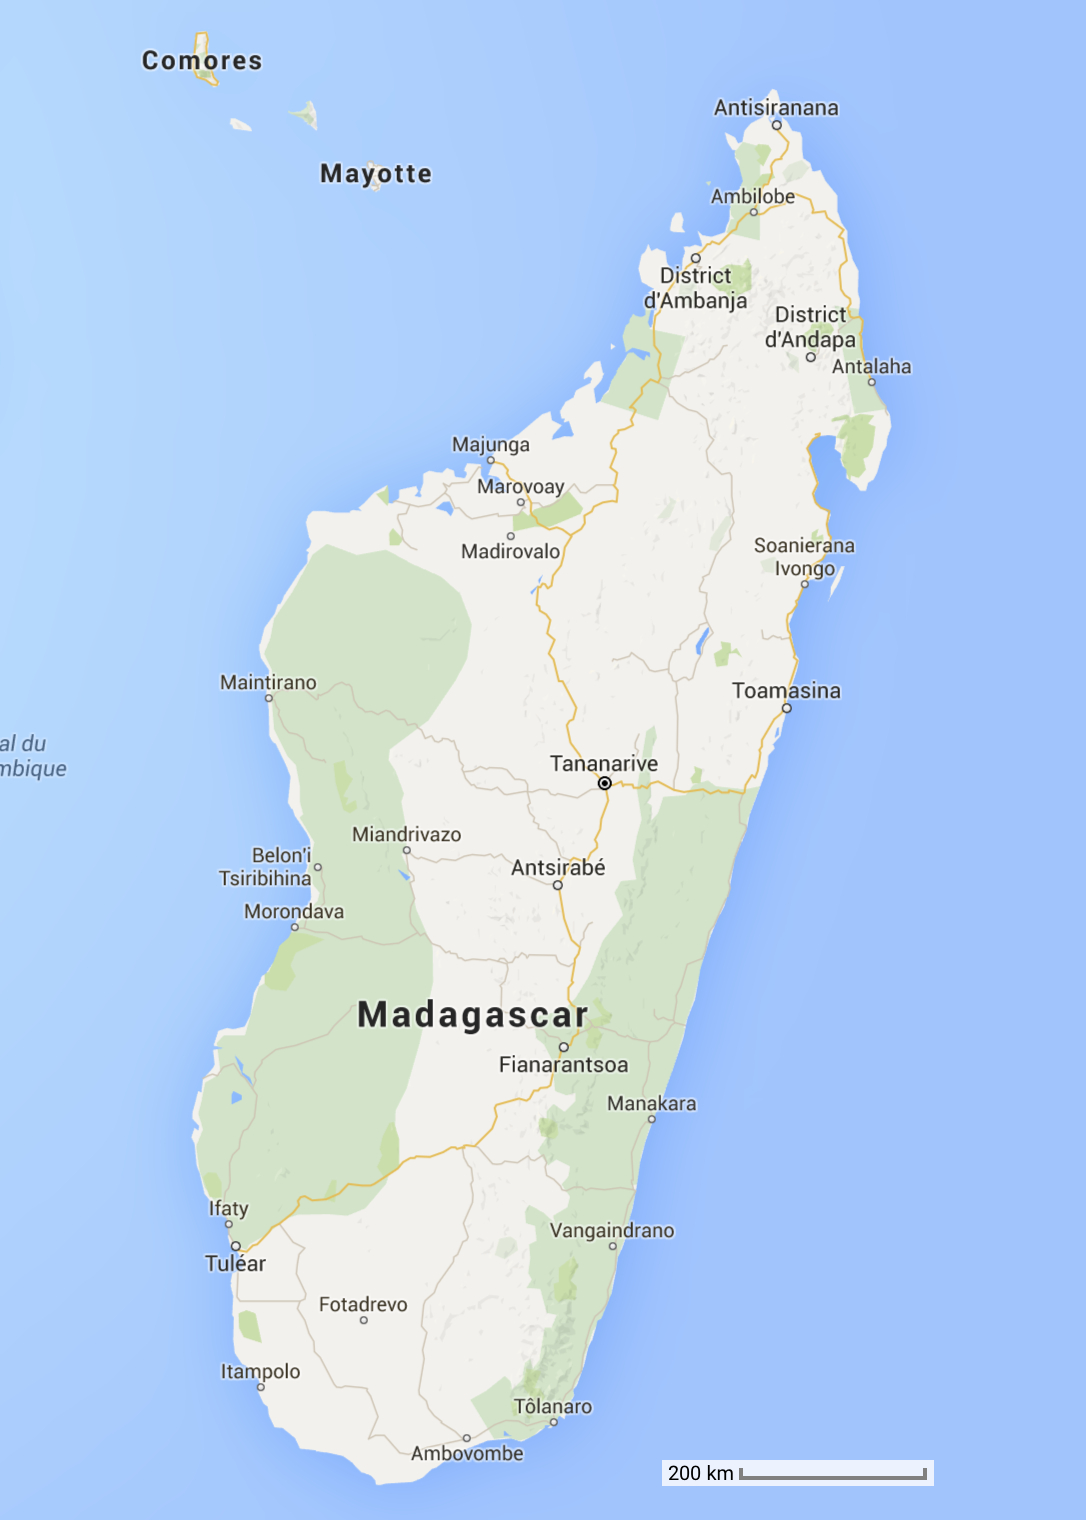
\includegraphics[width=4.8cm]{articles/Vous-etes-prets/madagascar.png}
Carte de Madagascar

Je vous laisse, il me reste quelques petite choses à boucler avant de partir, alors à bientôt et n'hésitez pas à laisser des commentaires sous les billets, ça fait toujours chaud au coeur de les lire.

Au revoir

\end{multicols}
